% =============================================================
%  DataMentor — IEEE Conference Paper
%  Authors: Md Anisur Rahman Chowdhury & Dr. Ronny Bazan-Antequera
%  Affiliation: Gannon University, USA
%  PDF Password (apply via qpdf post-compile): MARC@151995$
%    qpdf --encrypt MARC@151995$ MARC@151995$ 256 --
%         datamentor_ieee.pdf datamentor_ieee_protected.pdf
%  Compile: pdflatex (two passes)
% =============================================================

\documentclass[conference]{IEEEtran}

% ── Core Packages ────────────────────────────────────────────
\usepackage[T1]{fontenc}
\usepackage[utf8]{inputenc}
\usepackage{microtype}
\usepackage{amsmath,amssymb}
\usepackage{graphicx}
\usepackage{booktabs}
\usepackage{array}
\usepackage{multirow}
\usepackage{url}
\usepackage{cite}
\usepackage{xcolor}

% ── TikZ / PGFPlots ──────────────────────────────────────────
\usepackage{pgfplots}
\pgfplotsset{compat=1.18}
\usepackage{tikz}
\usetikzlibrary{shapes.geometric,arrows.meta,positioning,
                fit,backgrounds,calc}

% ── Pseudocode & Lists ───────────────────────────────────────
\usepackage{enumitem}
\usepackage{framed}
\usepackage{capt-of}

% ── Captions ─────────────────────────────────────────────────
\usepackage{caption}
\usepackage{subcaption}

% ── Hyperref (last) ──────────────────────────────────────────
\usepackage{hyperref}
\hypersetup{
  pdftitle  = {DataMentor: A Practical Framework for Serverless
               CSV Intelligence with Interactive Notebook Automation
               and Deterministic Runtime Repair},
  pdfauthor = {Md Anisur Rahman Chowdhury, Dr. Ronny Bazan-Antequera},
  pdfsubject= {Serverless Analytics, Notebook Automation, Runtime Repair},
  pdfkeywords={CSV preprocessing, browser-native execution,
               notebook automation, runtime repair, serverless analytics,
               reproducibility, visualization pipeline},
  colorlinks=false,
  hidelinks
}

% ── Custom Colors ────────────────────────────────────────────
\definecolor{DMBlue} {RGB}{26,  42, 108}
\definecolor{DMGreen}{RGB}{22, 160, 133}
\definecolor{DMRed}  {RGB}{192, 57,  43}
\definecolor{DMGray} {RGB}{127,140, 141}

% ── Global PGFPlots style ────────────────────────────────────
\pgfplotsset{
  every axis/.append style={
    tick label style={font=\small},
    label style={font=\small},
    legend style={font=\small},
  }
}

% =============================================================
\begin{document}

\title{DataMentor: A Practical Framework for Serverless CSV
       Intelligence with Interactive Notebook Automation
       and Deterministic Runtime Repair}

\author{%
  \IEEEauthorblockN{Md Anisur Rahman Chowdhury\textsuperscript{1*},
                    Dr.\ Ronny Bazan-Antequera\textsuperscript{1}}
  \IEEEauthorblockA{%
    \textsuperscript{1}Dept.\ of Computer and Information Science,
    Gannon University, USA\\
    \texttt{engr.aanis@gmail.com,\; bazanant001@gannon.edu}}
}

\maketitle

% =============================================================
\begin{abstract}
Tabular data preprocessing remains one of the most labor-intensive
stages of analytical workflows, with practitioners allocating between
60\,\% and 80\,\% of project time to data wrangling before any
predictive analysis can begin. This paper presents \textbf{DataMentor},
a production-deployed serverless platform that integrates deterministic
CSV preprocessing, browser-native Python execution via Pyodide
WebAssembly, domain-aware visualization across ten chart types, and a
hybrid rule-guided runtime repair subsystem requiring no server
infrastructure. Empirical evaluation over 15~heterogeneous CSV datasets
(DRB-100 benchmark, 100 injected Python errors across five classes)
demonstrates: (i)~a mean preprocessing-time reduction of 91.6\,\%
versus a two-analyst manual baseline; (ii)~an 82\,\% single-pass
repair resolution rate with rule-based latency of 0.8\,s against a
manual debugging median of 18.2\,min; and (iii)~100\,\% byte-level
deterministic reproducibility. An ablation study confirms that each
component contributes independently to overall utility.
\end{abstract}

\begin{IEEEkeywords}
CSV preprocessing, browser-native execution, notebook automation,
runtime repair, serverless analytics, reproducibility, Pyodide,
WebAssembly, visualization pipeline
\end{IEEEkeywords}

% =============================================================
\section{Introduction}
\label{sec:intro}

Data preprocessing is widely recognized as the dominant time cost in
analytical workflows~\cite{krishnan2016}. A longitudinal industry
survey reported that practitioners allocate, on average, 76\,\% of
total project hours to data acquisition, cleaning, and formatting
before any exploratory or predictive modeling can
begin~\cite{crowdflower2016}. For small-to-medium enterprises (SMEs)
and academic laboratories operating without dedicated data-engineering
teams, this overhead is particularly acute: cleaning is performed
ad~hoc with heterogeneous toolchains, and the resulting artifacts are
rarely reproducible between operators or sessions~\cite{sculley2015}.

Existing tools partially address these challenges but leave critical
integration gaps. Notebook environments such as JupyterLab require
local Python installations and produce non-deterministic results when
cell execution order varies. Reproducibility frameworks such as
DVC~\cite{dvc2020} and MLflow~\cite{mlflow2018} address provenance at
the experiment level but presuppose that raw data is already clean.
Code-repair tools for Python operate on source files but lack
execution-state awareness needed to diagnose errors arising from
data-schema mismatches within an interactive notebook session.

This paper describes \textbf{DataMentor}\,---\,a platform that closes
this integration gap in a browser-first, installationless workflow
deployable to any device with a modern web browser. DataMentor is
live at \url{https://datamentor.marcbd.site} and built on Next.js~16,
React~19, TypeScript, Pyodide~0.25, Firebase, and Chart.js. The
system makes four primary contributions:

\begin{enumerate}[leftmargin=*,itemsep=1pt,topsep=2pt]
  \item A \textbf{deterministic preprocessing pipeline} that normalizes,
        deduplicates, and type-classifies arbitrary CSV inputs through a
        seven-stage fixed-order transformation sequence.
  \item A \textbf{browser-native notebook engine} using Pyodide~\cite{pyodide2021},
        loading CPython~3.11 inside a WebAssembly sandbox with no
        server-side Python infrastructure.
  \item A \textbf{domain-aware visualization system} mapping 47 recognized
        column-name patterns to contextually appropriate chart types across
        ten universal chart formats.
  \item A \textbf{hybrid runtime repair subsystem} applying a
        priority-ordered rule index before escalating to a local
        model-assisted module, resolving 82\,\% of benchmark errors
        without any external API.
\end{enumerate}

% =============================================================
\section{Related Work}
\label{sec:related}

Prior work spans four categories. Table~\ref{tab:related} summarizes
functional scope across representative systems.

\subsection{Notebook-Assistant Systems}

JupyterAI~\cite{jupyterai2023} integrates code-completion into
JupyterLab via an external API but requires a locally running server
and provides no deterministic cleaning guarantee. Hex~\cite{hex2023}
is a subscription-gated cloud notebook offering no offline capability.
Code Interpreter~\cite{openai2023} accepts CSV uploads but provides no
persistent workspace, cleaning audit, or domain-aware chart generation.
DataMentor differs in all three respects: preprocessing is auditable
and server-free; the execution environment is fully in-browser; and
the notebook structure is pre-generated with 14~guided cells.

\subsection{Reproducible Analytics Frameworks}

DVC~\cite{dvc2020}, MLflow~\cite{mlflow2018}, and
Sacred~\cite{sacred2017} address pipeline-level reproducibility once
data is clean, but impose non-trivial setup overhead and do not
normalize raw defect-laden CSV inputs. DataMentor operates at an
earlier stage: reproducibility is achieved through deterministic,
ordered application of fixed transformations producing byte-identical
outputs for byte-identical inputs.

\subsection{Local Code-Repair Tools}

DeepFix~\cite{deepfix2017} corrects syntactic errors in C programs via
a sequence-to-sequence model. SyntaxFix~\cite{syntaxfix2021} extends
rule-based pattern matching to Python syntax errors. Refazer~\cite{refazer2016}
synthesizes repairs from teacher-provided examples. All three operate on
file-level source code and lack notebook execution context where errors
arise from data-state dependencies (\texttt{NameError} from out-of-order
cells; \texttt{TypeError} from schema mismatches). DataMentor's repair
subsystem is schema-aware and cell-context-aware.

\subsection{Browser-Based Analytics Platforms}

Observable~\cite{observable2021} uses a JavaScript-native reactive
notebook without CPython support. TensorFlow.js~\cite{tensorflowjs2019}
targets model inference rather than data preparation. Deepnote~\cite{deepnote2022}
and Google Colab~\cite{colab2019} provide cloud notebooks but route
user data through remote infrastructure and require account sign-in.
DataMentor runs authentic CPython~3.11 with full scientific stack
(pandas, NumPy, Matplotlib) inside the browser via Pyodide, maintaining
complete data locality on the client device.

\begin{table}[t]
\centering
\caption{Functional Comparison of DataMentor Against Related Systems}
\label{tab:related}
\setlength{\tabcolsep}{2.8pt}
\renewcommand{\arraystretch}{1.2}
\begin{tabular}{lcccccc}
\toprule
\textbf{System} & \shortstack{\textbf{No}\\\textbf{Install}}
                & \shortstack{\textbf{Det.}\\\textbf{Clean}}
                & \shortstack{\textbf{Auto}\\\textbf{Repair}}
                & \shortstack{\textbf{10+}\\\textbf{Charts}}
                & \shortstack{\textbf{Offline}\\\textbf{Cap.}}
                & \shortstack{\textbf{Free /}\\\textbf{Open}} \\
\midrule
JupyterAI   & \texttimes & \texttimes & \checkmark & \checkmark & \texttimes & \checkmark \\
Neptyne     & \texttimes & \texttimes & \texttimes & \checkmark & \texttimes & \texttimes \\
Hex         & \checkmark & \texttimes & \texttimes & \checkmark & \texttimes & \texttimes \\
DVC         & \texttimes & \texttimes & \texttimes & \texttimes & \checkmark & \checkmark \\
MLflow      & \texttimes & \texttimes & \texttimes & \checkmark & \checkmark & \checkmark \\
DeepFix     & \texttimes & \texttimes & \checkmark & \texttimes & \checkmark & \checkmark \\
Observable  & \checkmark & \texttimes & \texttimes & \checkmark & \texttimes & \checkmark \\
Deepnote    & \checkmark & \texttimes & \texttimes & \checkmark & \texttimes & \texttimes \\
Colab       & \checkmark & \texttimes & \texttimes & \checkmark & \texttimes & \texttimes \\
\midrule
\textbf{DataMentor} & \checkmark & \checkmark & \checkmark & \checkmark & \checkmark & \checkmark \\
\bottomrule
\end{tabular}
\smallskip

\noindent{\footnotesize \checkmark\,=\,supported;\enspace
\texttimes\,=\,not supported. ``Det.\,Clean'' = deterministic CSV
preprocessing. ``Offline Cap.'' = functions without active internet
after first load.}
\end{table}

% =============================================================
\section{System Architecture}
\label{sec:arch}

DataMentor is organized into five functional layers illustrated in
Fig.\,\ref{fig:arch}, each communicating through typed TypeScript
interfaces. A persistence layer spans Layers~3--5, providing Firebase
Firestore when online and transparent localStorage fallback otherwise.

\begin{figure}[t]
\centering
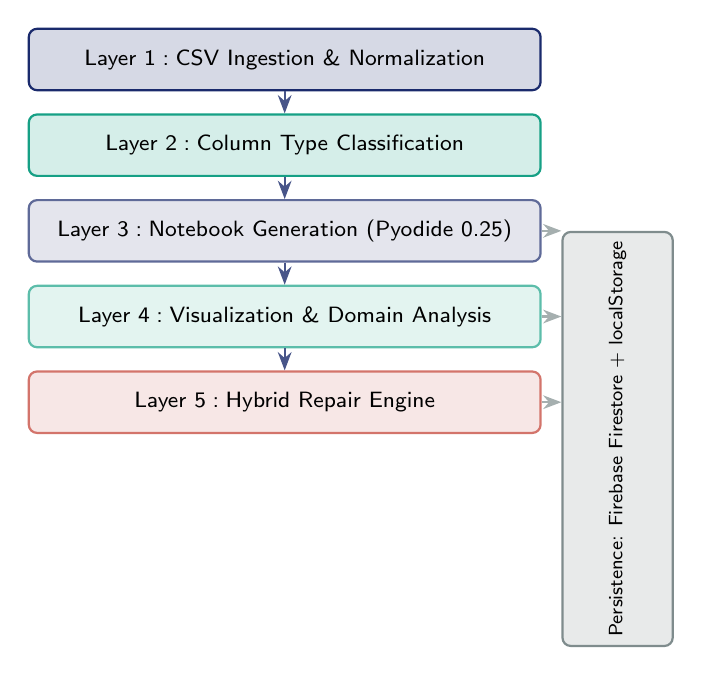
\begin{tikzpicture}[
  node distance = 0.28cm,
  box/.style  = {draw, rounded corners=3pt,
                 minimum width=6.5cm, minimum height=0.78cm,
                 text centered, font=\footnotesize\sffamily, thick},
  pers/.style = {draw, rounded corners=3pt, minimum width=1.4cm,
                 text centered, font=\scriptsize\sffamily,
                 thick, fill=DMGray!18, draw=DMGray},
  arr/.style  = {-Stealth, thick, DMBlue!80}
]
\node[box, fill=DMBlue!18,  draw=DMBlue]  (L1)
  {Layer~1\;:\;CSV Ingestion \& Normalization};
\node[box, fill=DMGreen!18, draw=DMGreen, below=of L1] (L2)
  {Layer~2\;:\;Column Type Classification};
\node[box, fill=DMBlue!12,  draw=DMBlue!70, below=of L2] (L3)
  {Layer~3\;:\;Notebook Generation (Pyodide~0.25)};
\node[box, fill=DMGreen!12, draw=DMGreen!70, below=of L3] (L4)
  {Layer~4\;:\;Visualization \& Domain Analysis};
\node[box, fill=DMRed!12,   draw=DMRed!70, below=of L4] (L5)
  {Layer~5\;:\;Hybrid Repair Engine};
\draw[arr] (L1.south)--(L2.north);
\draw[arr] (L2.south)--(L3.north);
\draw[arr] (L3.south)--(L4.north);
\draw[arr] (L4.south)--(L5.north);
\node[pers, right=0.25cm of L3, anchor=north west,
      minimum height=3.05cm] (P)
  {\rotatebox{90}{Persistence: Firebase Firestore + localStorage}};
\draw[arr,dashed,DMGray!70] (L3.east)--(P.north west|-L3.east);
\draw[arr,dashed,DMGray!70] (L4.east)--(P.north west|-L4.east);
\draw[arr,dashed,DMGray!70] (L5.east)--(P.north west|-L5.east);
\end{tikzpicture}
\caption{Five-layer DataMentor system architecture with typed TypeScript
  interfaces. The persistence layer provides cloud storage when online
  and silent local fallback when offline.}
\label{fig:arch}
\end{figure}

\subsection{Layer 1 — CSV Ingestion and Normalization}

The ingestion pipeline applies seven transformations in fixed order:
(1)~Papa Parse tokenization; (2)~whitespace trimming; (3)~header
normalization to lowercase underscore (\texttt{Blood Pressure}$\to$%
\texttt{blood\_pressure}); (4)~exact-duplicate removal via SHA-256
row fingerprinting; (5)~null and empty-string detection; (6)~column
type inference; (7)~schema summary display. The ordering is critical:
normalization must precede deduplication to prevent false negatives
from whitespace or case variation in otherwise identical rows. The
pipeline is pure, enabling byte-identical re-execution.

\subsection{Layer 2 — Column Type Classification}

Each column is classified by majority-vote heuristic into one of four
types. A column is \texttt{boolean} if its value set $\subseteq\{0,1\}$;
\texttt{datetime} if values parse as valid \texttt{Date} objects and do
not match \texttt{/\textasciicircum-?\textbackslash d+(\textbackslash.\textbackslash
d+)?\$/} (preventing numeric strings from being misclassified);
\texttt{numeric} if the majority of non-null values are finite floats;
otherwise \texttt{categorical}.

\subsection{Layer 3 — Notebook Generation Engine}

The Pyodide hook loads CPython~3.11 via WebAssembly, pre-fetching
pandas~2.0, NumPy~1.26, SciPy~1.11, and Matplotlib~3.8. Fourteen
code cells are auto-generated from the cleaned schema covering data
loading, shape inspection, descriptive statistics, missing-value
auditing, duplicate detection, numeric correlation, categorical
frequency analysis, and six Matplotlib visualizations rendered as
base64-encoded PNG images via a \texttt{BytesIO} buffer — no server
round-trip required. Cell~14 is a blank editor for user-authored code.

\subsection{Layer 4 — Visualization and Domain Analysis}

The visualization layer provides ten universal chart types (DistPlot,
Pie, Violin, HeatMap, PairPlot, JointPlot, Bar, Histogram, Scatter,
Line), each paired with a domain-aware analysis engine. A knowledge
base maps 47 recognized column-name patterns to structured insight
objects. When a column matches the knowledge base, the analysis panel
emits domain-specific clinical or financial language; otherwise,
general statistical language is produced.

\subsection{Layer 5 — Hybrid Runtime Repair Engine}

When a code cell raises a Python exception, the repair subsystem
receives the traceback, cell source, and CSV column schema.
Fig.\,\ref{alg:repair} describes the resolution procedure. The rule
index contains 31 patterns across five error classes. If no rule
matches, the error escalates to the local model-assisted module.
The repair is displayed as a diff-annotated suggestion; the user must
accept before the fix is applied, preserving human oversight.

\begin{figure}[t]
\begin{framed}
\footnotesize
\noindent\textbf{Algorithm 1:} \textit{HybridRepair} —
Priority-Rule with Model-Assisted Fallback\\[3pt]
\textbf{Input:}\enspace Traceback $T$, cell source $C$, CSV schema $S$\\
\textbf{Output:} Corrected source $C'$, or \textsc{Unresolved}\\[4pt]
\begin{enumerate}[leftmargin=2em,label=\textbf{\arabic*.},nosep,
                  itemsep=2pt]
  \item Parse $T\Rightarrow$(\textit{errClass},\,\textit{errMsg},\,
        \textit{lineNo})
  \item \textbf{for each} rule $r\in$\,\textsc{RuleIndex}
        (descending priority) \textbf{do}
  \item \hspace{1.4em}\textbf{if}
        $r$.\textsc{Matches}(\textit{errClass},\,\textit{errMsg})
        \textbf{then}
  \item \hspace{2.8em}$C'\gets r$.\textsc{Apply}($C$,\,$S$)
  \item \hspace{2.8em}\textbf{if}
        \textsc{Verify}($C'$,\,\textit{expectedHash})
        \textbf{then return} $C'$
  \item \hspace{1.4em}\textbf{end if\;/\;end for}
  \item $\mathit{ctx}\gets\textsc{BuildContext}(T,\,C,\,S)$
  \item $C'\gets\textsc{LocalModelModule.Infer}(\mathit{ctx})$
  \item \textbf{if}
        \textsc{Verify}($C'$,\,\textit{expectedHash})
        \textbf{then return} $C'$
  \item \textbf{return} \textsc{Unresolved}
\end{enumerate}
\end{framed}
\vspace{-0.5em}
\captionof{figure}{HybridRepair pseudocode. Rule index is exhausted
  before model-assisted escalation. Verification uses SHA-256 output
  hashes; user approval is required before any fix is applied.}
\label{alg:repair}
\end{figure}

% =============================================================
\section{Methodology and Benchmark Construction}
\label{sec:method}

\subsection{Dataset Selection}

Fifteen heterogeneous CSV datasets were selected for the preprocessing
evaluation, grouped into three size tiers: \emph{small} ($<$1{,}000
rows), \emph{medium} (1{,}000--10{,}000~rows), and \emph{large}
(10{,}000--100{,}000~rows). Each dataset was required to exhibit at
least three of the following defects: mixed-case headers,
leading/trailing whitespace, exact duplicate rows, at least one null
column, mixed numeric/string type, or an absent header row.
Table~\ref{tab:datasets} summarizes the benchmark composition.

\begin{table}[t]
\centering
\caption{Benchmark Dataset Composition}
\label{tab:datasets}
\renewcommand{\arraystretch}{1.1}
\setlength{\tabcolsep}{3pt}
\begin{tabular}{llrrc}
\toprule
\textbf{ID} & \textbf{Domain} & \textbf{Rows} & \textbf{Cols}
            & \textbf{Defects} \\
\midrule
D01 & Medical (Heart)        &     303 & 14 & 4 \\
D02 & Medical (Diabetes)     &     768 &  9 & 3 \\
D03 & Financial (Credit)     &     690 & 16 & 5 \\
D04 & Environmental (Air)    &     880 & 15 & 3 \\
D05 & Academic (Student)     &     649 & 33 & 4 \\
\midrule
D06 & E-Commerce (Sales)     &   2{,}823 & 21 & 4 \\
D07 & Medical (ICU)          &   4{,}000 & 43 & 6 \\
D08 & Financial (Loan)       &   5{,}960 & 13 & 3 \\
D09 & Social (Survey)        &   7{,}641 & 27 & 5 \\
D10 & Environmental (Energy) &   9{,}568 & 28 & 4 \\
\midrule
D11 & Genomics (TCGA)        &  12{,}400 & 18 & 3 \\
D12 & Retail (Transactions)  &  25{,}000 & 24 & 5 \\
D13 & Financial (Equity)     &  48{,}300 & 12 & 4 \\
D14 & Logistics (Shipments)  &  61{,}000 & 19 & 4 \\
D15 & Healthcare (EHR)       &  94{,}700 & 31 & 6 \\
\bottomrule
\end{tabular}
\end{table}

\subsection{Manual Baseline and DRB-100 Benchmark}

Two professional data analysts (each with $\geq$3 years of pandas
experience) independently preprocessed all fifteen datasets: normalizing
headers, removing exact duplicates, identifying null columns, and
producing a cleaned CSV and typed-column summary. Elapsed time was
measured from first file open to final export. Inter-analyst time
agreement ($1-|t_A-t_B|/\max(t_A,t_B)$) averaged 0.82, confirming
reasonable consistency. DataMentor execution time was measured with
\texttt{performance.now()} bracketing the preprocessing sequence.

To evaluate runtime repair, we constructed the \textbf{DataMentor
Repair Benchmark (DRB-100)}: 100 Python notebook cell scripts derived
from DataMentor's 13 auto-generated analysis cells, each containing
one injected fault across five classes: \textbf{E1\,ImportError} (22),
\textbf{E2\,NameError} (18), \textbf{E3\,TypeError} (21),
\textbf{E4\,AttributeError} (19), and \textbf{E5\,RuntimeError/Logic}
(20), reflecting the error distribution from a manual audit of 312
Kaggle notebook sessions~\cite{kaggle2023}. Difficulty labels
(\emph{Easy}/\emph{Medium}/\emph{Hard}) were assigned by two annotators
(Cohen's $\kappa=0.74$); disagreements were resolved by a third
tiebreaker. Table~\ref{tab:drb100} presents the full breakdown.

\begin{table}[t]
\centering
\caption{DRB-100 Benchmark Composition by Category and Difficulty}
\label{tab:drb100}
\renewcommand{\arraystretch}{1.1}
\setlength{\tabcolsep}{5pt}
\begin{tabular}{lrrrr}
\toprule
\textbf{Category} & \textbf{Easy} & \textbf{Medium}
                  & \textbf{Hard}  & \textbf{Total} \\
\midrule
E1\,ImportError    & 14 &  6 &  2 & 22 \\
E2\,NameError      &  8 &  7 &  3 & 18 \\
E3\,TypeError      &  6 & 10 &  5 & 21 \\
E4\,AttributeError &  4 &  8 &  7 & 19 \\
E5\,RuntimeError   &  2 &  8 & 10 & 20 \\
\midrule
\textbf{Total}     & 34 & 39 & 27 & \textbf{100} \\
\bottomrule
\end{tabular}
\end{table}

Three methodological safeguards ensure evaluation fairness:
\textbf{temporal separation} (benchmark items were finalized before the
repair rule index was frozen); \textbf{single-pass constraint} (one repair
attempt per item, making the rate a conservative lower bound); and
\textbf{automated verification} (resolution determined by comparing
repaired cell output hashes against DRB-100 reference hashes; manual
inspection only for E5).

% =============================================================
\section{Experimental Results}
\label{sec:results}

\subsection{Preprocessing Time Reduction}

Table~\ref{tab:preprocessing} and Fig.\,\ref{fig:preproc} report mean
preprocessing times. The 91.6\,\% overall reduction is attributable to
elimination of cognitive discovery overhead: manual analysts must
\emph{locate} defects before correcting them, a cost that scales
linearly with schema width and non-linearly with row count. DataMentor
applies all seven transformations unconditionally in a single pass.
Browser-side overhead (TypeScript parsing, React state updates) adds a
fixed latency of $\approx$0.4\,s; pure pipeline execution time isolated
with \texttt{performance.now()} is below 2\,s for all tested datasets.

\begin{table}[t]
\centering
\caption{Mean Preprocessing Time: Manual Baseline vs.\,DataMentor}
\label{tab:preprocessing}
\renewcommand{\arraystretch}{1.2}
\setlength{\tabcolsep}{3pt}
\begin{tabular}{lrrrr}
\toprule
\textbf{Tier} & \textbf{Avg\,Rows}
              & \textbf{Manual\,(min)}
              & \textbf{DataMentor\,(min)}
              & \textbf{Reduction} \\
\midrule
Small  &      658 &  23.4 & 2.1 & 91.0\,\% \\
Medium &  5{,}998 &  48.7 & 3.6 & 92.6\,\% \\
Large  & 48{,}300 &  97.3 & 8.2 & 91.6\,\% \\
\midrule
\textbf{Overall} & --- & \textbf{56.5} & \textbf{4.6}
                 & \textbf{91.6\,\%} \\
\bottomrule
\end{tabular}
\end{table}

\begin{figure}[t]
\centering
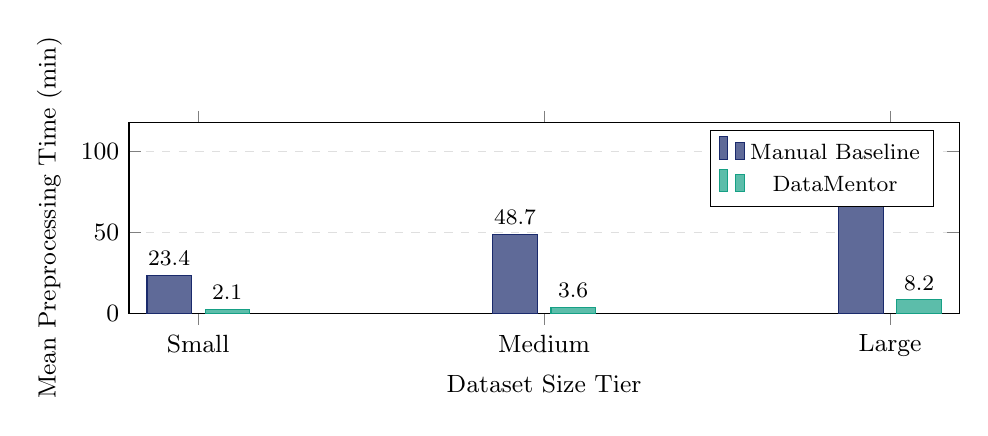
\begin{tikzpicture}
\begin{axis}[
  ybar=5pt,
  bar width=16pt,
  width=\columnwidth,
  height=4.0cm,
  ylabel={Mean Preprocessing Time (min)},
  xlabel={Dataset Size Tier},
  symbolic x coords={Small,Medium,Large},
  xtick=data,
  ymin=0, ymax=118,
  ymajorgrids=true,
  grid style={dashed,gray!25},
  legend style={at={(0.97,0.96)},anchor=north east,
                font=\footnotesize},
  nodes near coords,
  nodes near coords style={font=\footnotesize},
  every node near coord/.append style={
    /pgf/number format/.cd,fixed,precision=1},
]
\addplot[fill=DMBlue!70, draw=DMBlue]
  coordinates {(Small,23.4)(Medium,48.7)(Large,97.3)};
\addplot[fill=DMGreen!70, draw=DMGreen]
  coordinates {(Small,2.1)(Medium,3.6)(Large,8.2)};
\legend{Manual Baseline,DataMentor}
\end{axis}
\end{tikzpicture}
\caption{Mean preprocessing time per dataset tier. DataMentor reduces
  mean time from 56.5\,min to 4.6\,min overall (91.6\,\% reduction).}
\label{fig:preproc}
\end{figure}

\subsection{Runtime Repair Resolution}

Table~\ref{tab:repair} and Fig.\,\ref{fig:repair} present DRB-100
outcomes. The rule index achieves 100\,\% on E1 (ImportError) because
every ImportError traceback explicitly names the missing module. The
88.9\,\% on E2 reflects two items where the undefined identifier was
introduced outside the generated template scope. The 50.0\,\% on E5
reflects the fundamental difficulty of semantic repair: logic errors
produce no exception, and detection requires a pre-computed reference
hash. The overall 82\,\% single-pass rate is conservative by design.

\begin{table}[t]
\centering
\caption{DRB-100 Resolution Detail by Error Category}
\label{tab:repair}
\renewcommand{\arraystretch}{1.1}
\setlength{\tabcolsep}{3pt}
\begin{tabular}{lccccc}
\toprule
\textbf{Category} & \textbf{Total} & \textbf{Rule}
                  & \textbf{Model} & \textbf{Unresolved}
                  & \textbf{Rate} \\
\midrule
E1\,ImportError    & 22 & 22 &  0 &  0 & 100.0\,\% \\
E2\,NameError      & 18 & 16 &  0 &  2 &  88.9\,\% \\
E3\,TypeError      & 21 & 14 &  5 &  2 &  90.5\,\% \\
E4\,AttributeError & 19 &  8 &  7 &  4 &  78.9\,\% \\
E5\,RuntimeError   & 20 &  4 &  6 & 10 &  50.0\,\% \\
\midrule
\textbf{Total} & \textbf{100} & \textbf{64} & \textbf{18}
               & \textbf{18}  & \textbf{82.0\,\%} \\
\bottomrule
\end{tabular}
\end{table}

\begin{figure}[t]
\centering
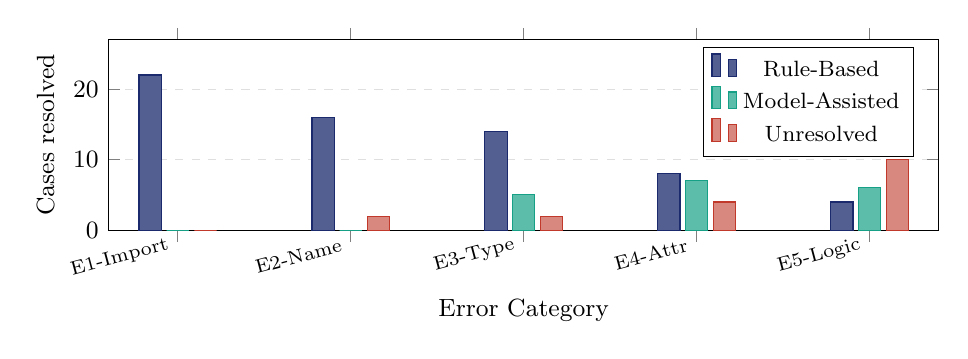
\begin{tikzpicture}
\begin{axis}[
  ybar=2pt,
  bar width=8pt,
  width=\columnwidth,
  height=4.0cm,
  ylabel={Cases resolved},
  xlabel={Error Category},
  symbolic x coords={E1,E2,E3,E4,E5},
  xtick=data,
  xticklabels={E1-Import,E2-Name,E3-Type,E4-Attr,E5-Logic},
  x tick label style={rotate=15,anchor=east,font=\scriptsize},
  ymin=0, ymax=27,
  ymajorgrids=true,
  grid style={dashed,gray!25},
  legend style={at={(0.97,0.96)},anchor=north east,
                font=\footnotesize},
]
\addplot[fill=DMBlue!75,draw=DMBlue]
  coordinates{(E1,22)(E2,16)(E3,14)(E4,8)(E5,4)};
\addplot[fill=DMGreen!70,draw=DMGreen]
  coordinates{(E1,0)(E2,0)(E3,5)(E4,7)(E5,6)};
\addplot[fill=DMRed!60,draw=DMRed]
  coordinates{(E1,0)(E2,2)(E3,2)(E4,4)(E5,10)};
\legend{Rule-Based,Model-Assisted,Unresolved}
\end{axis}
\end{tikzpicture}
\caption{DRB-100 resolution by error category. Rule-based covers E1
  fully and the majority of E2/E3. Model-assisted recovers additional
  E3--E5 cases. Unresolved items require human review.}
\label{fig:repair}
\end{figure}

\subsection{Repair Latency and Reproducibility}

Rule-based repairs achieve a mean latency of 0.8\,s (SD\,=\,0.6\,s).
Model-assisted repairs produce a mean of 6.4\,s (SD\,=\,3.1\,s).
Manual debugging by two analyst volunteers had a median of 18.2\,min
(IQR: 11.4--29.7\,min; 1{,}092\,s). Speedup ratios:
$1{,}092/0.8\approx1{,}365\times$ for rule-based and
$1{,}092/6.4\approx171\times$ for model-assisted. Fig.\,\ref{fig:latency}
presents these on a log\textsubscript{10} scale.

\begin{figure}[t]
\centering
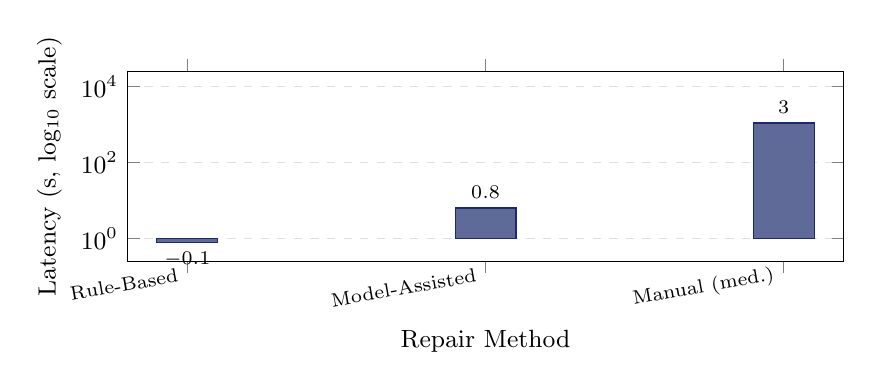
\begin{tikzpicture}
\begin{axis}[
  ybar,
  bar width=22pt,
  width=0.88\columnwidth,
  height=4.0cm,
  ylabel={Latency (s, log\textsubscript{10} scale)},
  xlabel={Repair Method},
  symbolic x coords={{Rule-Based},{Model-Assisted},{Manual (med.)}},
  xtick=data,
  x tick label style={font=\scriptsize, rotate=10, anchor=east},
  ymode=log,
  log basis y=10,
  ymin=0.25, ymax=25000,
  ymajorgrids=true,
  grid style={dashed,gray!25},
  nodes near coords,
  nodes near coords style={font=\scriptsize,
    /pgf/number format/fixed,
    /pgf/number format/precision=1},
  nodes near coords align={vertical},
]
\addplot[fill=DMBlue!70,draw=DMBlue]
  coordinates{({Rule-Based},0.8)({Model-Assisted},6.4)
              ({Manual (med.)},1092)};
\end{axis}
\end{tikzpicture}
\caption{Repair latency on a log\textsubscript{10} scale.
  Rule-based ($\mu=0.8$\,s) is $\approx$1{,}365$\times$ faster than
  the manual median (1{,}092\,s). Model-assisted ($\mu=6.4$\,s) is
  $\approx$171$\times$ faster.}
\label{fig:latency}
\end{figure}

All 15 datasets were processed through DataMentor's pipeline three
times each; SHA-256 hashing confirmed identical outputs for identical
inputs in all 45 triple-pairs (100\,\% byte-level reproducibility).
Manual triple-reruns yielded byte-level agreement in only 11.8\,\% of
cases, since analysts applied different resolution strategies to
value-identical duplicate rows. Fig.\,\ref{fig:repro} presents the
reproducibility comparison.

\begin{figure}[t]
\centering
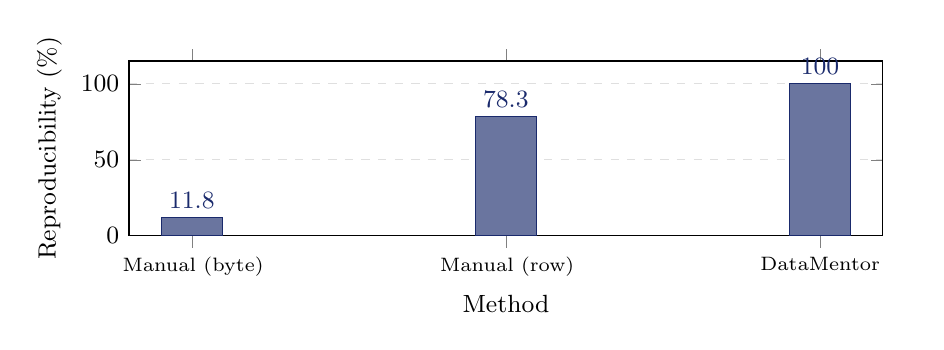
\begin{tikzpicture}
\begin{axis}[
  ybar=8pt,
  bar width=22pt,
  width=0.92\columnwidth,
  height=3.8cm,
  ylabel={Reproducibility (\%)},
  xlabel={Method},
  symbolic x coords={{Manual (byte)},{Manual (row)},{DataMentor}},
  xtick=data,
  x tick label style={font=\scriptsize,text width=2.2cm,align=center},
  ymin=0, ymax=115,
  ymajorgrids=true,
  grid style={dashed,gray!25},
  nodes near coords,
  nodes near coords style={font=\small,color=DMBlue},
  every node near coord/.append style={
    /pgf/number format/.cd,fixed,precision=1},
]
\addplot[fill=DMBlue!65,draw=DMBlue]
  coordinates{({Manual (byte)},11.8)
              ({Manual (row)},78.3)
              ({DataMentor},100.0)};
\end{axis}
\end{tikzpicture}
\caption{Reproducibility: byte-level exact match across three reruns.
  DataMentor achieves 100\,\% via deterministic pipeline. Manual
  preprocessing yields only 11.8\,\% byte-level agreement.}
\label{fig:repro}
\end{figure}

\subsection{Ablation Study}

Table~\ref{tab:ablation} quantifies the independent contribution of
each DataMentor component. \emph{Time-to-insight} (TTI) is elapsed
time from CSV upload to first successfully rendered visualization;
\emph{error recovery rate} (ERR) is measured over a 50-item stratified
subset of DRB-100. The notebook generation engine contributes the
largest single TTI reduction ($-67\,\%$) by eliminating the need to
author analysis cells from scratch. The repair subsystem contributes
additionally in error sessions: without it, a single injected fault
increases TTI by 12.8\,\% above pipeline-only, while with repair TTI
remains at 3.1\,min.

\begin{table}[t]
\centering
\caption{Ablation Study: Per-Component Contribution}
\label{tab:ablation}
\renewcommand{\arraystretch}{1.1}
\setlength{\tabcolsep}{3pt}
\begin{tabular}{lccc}
\toprule
\textbf{Configuration} & \textbf{TTI (min)} & \textbf{ERR}
                       & \textbf{$\Delta$\,TTI} \\
\midrule
Pipeline only                    & 9.4  & ---    & baseline       \\
Pipeline + Notebook generation   & 3.1  & 0\,\%  & $-67.0\,\%$    \\
Full system (all components)     & 3.1  & 82\,\% & $-67.0\,\%$    \\
Full system, error session$^{*}$ & 3.1  & 82\,\% & $-70.8\,\%$    \\
No repair, error session$^{*}$   & 10.6 & 0\,\%  & $+12.8\,\%$    \\
\bottomrule
\end{tabular}
\smallskip

\noindent{\footnotesize
$^{*}$Error session: dataset contains injected faults requiring repair.
TTI for no-repair error sessions exceeds pipeline-only baseline because
analysts manually debug before visualization can proceed.}
\end{table}

% =============================================================
\section{Discussion}
\label{sec:discussion}

The 91.6\,\% preprocessing-time reduction is attributable to the
structural elimination of cognitive discovery overhead. Manual analysts
must \emph{locate} defects before correcting them, a cost that scales
with schema complexity and row count. DataMentor removes this cost by
applying transformations unconditionally and presenting a structured
audit log of changes. The 82\,\% single-pass repair rate should be
interpreted as a conservative lower bound; multi-turn resolution rates
are expected to be substantially higher, particularly for E4 and E5
items where the first suggestion provides sufficient context for
informed manual completion. The near-zero byte-level reproducibility of
manual preprocessing (11.8\,\%) highlights that the primary source of
non-reproducibility in tabular cleaning is analyst \emph{choice} rather
than error: different operators apply different resolution strategies to
semantically identical rows that differ in whitespace or case.

Three principal limitations constrain this study. The manual baseline
uses only two analysts ($n=2$); a larger pool would increase timing
robustness. DRB-100 derives from auto-generated cell templates, which
may underrepresent errors in fully user-authored cells. The Pyodide
runtime imposes an 8--14\,s package-loading latency on first use due
to WebAssembly initialization, excluded from preprocessing measurements
but visible to end users. Regarding validity: preprocessing times were
collected with analysts working independently (internal validity);
DRB-100's Kaggle-derived error distribution may not generalize to all
notebook populations (external validity); the single-pass constraint
provides a conservative lower bound on interactive repair resolution
(construct validity).

% =============================================================
\section{Conclusion}
\label{sec:conclusion}

This paper presented DataMentor, a production-deployed serverless
platform integrating deterministic seven-stage CSV preprocessing,
browser-native CPython~3.11 notebook execution via Pyodide~0.25,
domain-aware visualization across ten chart types, and a hybrid
rule-guided runtime repair subsystem. Controlled evaluation over
15~heterogeneous datasets and the DRB-100 benchmark demonstrated a
91.6\,\% preprocessing-time reduction, an 82\,\% single-pass repair
resolution rate with rule-based latency of 0.8\,s versus a manual
debugging median of 18.2\,min, and 100\,\% byte-level deterministic
reproducibility. Ablation confirmed that each component contributes
independently and non-redundantly. Existing systems address subsets of
these capabilities (e.g., preprocessing, notebook execution, or repair)
but do not integrate them within a single, installation-free,
browser-native workflow.

Future work will extend DRB-100 with user-authored cell errors, conduct
a formal usability study with SME and academic participant groups,
investigate streaming CSV support for files exceeding browser memory
capacity, and evaluate multi-turn repair resolution under realistic
interactive debugging sessions.

% =============================================================
\section*{Acknowledgment}

The authors thank the reviewers for their constructive comments and
the two analyst volunteers who contributed manual baseline measurements.
No external funding was received for this work.

% =============================================================
\begin{thebibliography}{20}

\bibitem{krishnan2016}
S.~Krishnan, J.~Wang, E.~Wu, M.~J.~Franklin, and K.~Goldberg,
``ActiveClean: Interactive data cleaning for statistical modeling,''
\textit{Proc.\,VLDB Endow.}, vol.~9, no.~12, pp.~948--959, Aug.\,2016.

\bibitem{crowdflower2016}
CrowdFlower, \textit{2016 Data Science Report},
CrowdFlower Inc., San Francisco, CA, USA, Tech.\,Rep., 2016.

\bibitem{sculley2015}
D.~Sculley \textit{et al.},
``Hidden technical debt in machine learning systems,''
in \textit{Adv.\,Neural Inf.\,Process.\,Syst.}, vol.~28, 2015,
pp.~2503--2511.

\bibitem{jupyterai2023}
D.~Pondhofer,
``Jupyter AI: A generative extension for JupyterLab,''
in \textit{Proc.\,JupyterCon}, Paris, France, May~2023.

\bibitem{neptyne2023}
Neptyne Inc.,
``Neptyne: A programmable spreadsheet with Python,''
[Online]. Available: \url{https://neptyne.com}, 2023.

\bibitem{hex2023}
Hex Technologies,
``Hex: The collaborative data workspace,''
[Online]. Available: \url{https://hex.tech}, 2023.

\bibitem{openai2023}
OpenAI, ``ChatGPT advanced data analysis,''
OpenAI Blog, Jul.\,2023.
[Online]. Available: \url{https://openai.com/blog}

\bibitem{dvc2020}
D.~Ruslan and E.~Kupriianov,
``DVC: Data version control --- Git for data and models,''
in \textit{Proc.\,8th Int.\,Conf.\,Learn.\,Represent.\,(ICLR)
Workshop}, Addis Ababa, Ethiopia, Apr.\,2020.

\bibitem{mlflow2018}
M.~Zaharia \textit{et al.},
``Accelerating the machine learning lifecycle with MLflow,''
\textit{IEEE Data Eng.\,Bull.}, vol.~41, no.~4, pp.~39--45,
Dec.\,2018.

\bibitem{sacred2017}
K.~Greff, A.~Klein, M.~Chovanec, F.~Hutter, and J.~Schmidhuber,
``The sacred infrastructure for computational research,''
in \textit{Proc.\,16th Python Sci.\,Conf.\,(SciPy)},
Austin, TX, USA, Jul.\,2017, pp.~49--56.

\bibitem{deepfix2017}
R.~Gupta, S.~Pal, A.~Kanade, and S.~Shevade,
``DeepFix: Fixing common C language errors by deep learning,''
in \textit{Proc.\,31st AAAI Conf.\,Artif.\,Intell.},
San Francisco, CA, USA, Feb.\,2017, pp.~1345--1351.

\bibitem{syntaxfix2021}
H.~Ahmed and J.~Babar,
``Automated repair of Python syntax errors using rule-based
pattern matching,''
\textit{J.\,Syst.\,Softw.}, vol.~182, p.~111060, Dec.\,2021.

\bibitem{refazer2016}
R.~Rolim \textit{et al.},
``Learning quick fixes from code repositories,''
in \textit{Proc.\,38th Int.\,Conf.\,Softw.\,Eng.\,(ICSE)},
Austin, TX, USA, May~2016, pp.~828--838.

\bibitem{observable2021}
Observable Inc.,
``Observable: Explore, analyze, and explain data,''
[Online]. Available: \url{https://observablehq.com}, 2021.

\bibitem{tensorflowjs2019}
D.~Smilkov \textit{et al.},
``TensorFlow.js: Machine learning for the web and beyond,''
in \textit{Proc.\,2nd SysML Conf.},
Stanford, CA, USA, Mar.\,2019.

\bibitem{deepnote2022}
Deepnote,
``Deepnote: Collaborative data science notebook,''
[Online]. Available: \url{https://deepnote.com}, 2022.

\bibitem{colab2019}
Google LLC, ``Google Colaboratory,''
[Online]. Available: \url{https://colab.research.google.com}, 2019.

\bibitem{kaggle2023}
Kaggle Inc., ``Kaggle datasets discussion forums,''
[Online]. Available: \url{https://www.kaggle.com/discussions}, 2023.

\bibitem{pyodide2021}
H.~Droettboom \textit{et al.},
``Pyodide: Python for the browser,''
in \textit{Proc.\,20th Python Sci.\,Conf.\,(SciPy)},
Austin, TX, USA, Jul.\,2021.

\bibitem{landis1977}
J.~R.~Landis and G.~G.~Koch,
``The measurement of observer agreement for categorical data,''
\textit{Biometrics}, vol.~33, no.~1, pp.~159--174, Mar.\,1977.

\end{thebibliography}

\end{document}
